\newpage
\setlength{\columnsep}{50pt}
\begin{multicols}{2}
\setcounter{page}{37}
В школьном курсе математики свойствам элементарных неравенств и методам их доказательства отводится значительно место. Однако на вступительных экзаменах в вузы многие абитуриенты с трудом применяют неравенства при исследовании элементарных функций и решении задач на максимум и минимум (преимущественно геометрического и физического содержания). Между тем, для решения подобных задач достаточно знать и, главно, уметь применять сравнительно несложные неравенства.\par 
К числу таких неравенств относится, прежде всего, неравенство Коши: среднее арифмитическое двух положительных чисел a и b не меньше их среднего геометрического:
\begin{equation}\label{(1)}
    \frac{a+b}{2}\geq\sqrt[3]{ab}
\end{equation}
\[ \frac{a+b}{2}\geq\sqrt[3]{ab}\]
Наряду с неравенством Коши абитуриентам полезно знать некоторые следствия из него, а именно:
\begin{equation}
    a+b\geq2\sqrt{ab}
\end{equation}
\begin{equation}\label{(3)}
   a^2+b^2\geq2ab
\end{equation}
\begin{equation}\label{(4)}
    ab\leq(\frac{a+b}{2})
\end{equation}
\begin{equation}\label{(5)}
    ab\leq\frac{1}{2}(a^2+b^2)
\end{equation}
(выведите их самостоятельно).\par
Как известно, в неравенстве \eqref{1} равенство достигается лишь при \(a=b\). Следовательно, и неравенства \eqref{2}-\eqref{5} переходят в равенства лишь при \(a=b\). 

Неравенства \eqref{1}--\eqref{5} эквивалентны друг другу (при \(a>0, b>0\)), любое из них можно применять при решении задач, и, как показывает практика вступительных экзаменов, решение конкурсных задач на максимум и минимум легко находится именно с помощью этих неравенств. Рассмотрим ряд примеров.

\textsc{Задача 1.} \textit{Найти наибольшее значение произведения двух переменных, сумма которых постоянна.}

Этот вопрос решает неравенство \eqref{4}, утверждающее, что произведение двух положительных чисел не больше квадрата их среднего арифмитического. Действительно, если \(a\) и \(b\)--две переменные, \(a+b=M\), где \(M\)--некоторая постояная, то при \(a \neq b\) согласно \eqref{4} \(ab<(\frac{M}{2})^2\), а при \(a=b\) неравенство \eqref{4} переходит в равенство \(ab=(\frac{M}{2})^2\)

Аналогично, если требуется найти наименьшее значение суммы двух переменных, произведение которых постоянно, то применяется неравенство \eqref{2}

\textsc{Задача 2.} (МГУб мехмат 1966). \textit{Из гранита нужно вырубить постамент в форме прямоугольного параллелепипеда, высота которого должна быть равна диагонали основания, а площадь основания должна быть равна 4 \(m^2\). При каких длинах сторон основания площадь поверхности постамента будет наименьшей?}

Пусть \(x\) и \(y\) -- длины (в метрах) сторон прямоугольника, лежащего в основании постамента. Тогда по условию задачи высота \(z\) постамента равна \(\sqrt{x^2+y^2}\), а площадь его поверхности (в \(m^2\))
\[S = 2(x+y)\cdot\sqrt{x^2+y^2} + 8\]
при этом xy = 4. Воспользовавшись неравенствами (2) и (3), получим \(x+y\geq2\sqrt{xy} = 4; x^2 + y^2 \geq 2xy = 8,\)откуда \(\sqrt{x^2+y^2}\geq\sqrt{8}\)

Расмотрим как и раньше равенство
\[N=p_1^{a_1}p_2^{a_2}...p_k^{a_k}\]
с различными простыми \(p_1,p_2...,p_k\) и натуральными показателями \(\alpha_1, \alpha_2,...,\alpha_k\)
(Такое представление называется каноническим разложением числа \tetit{N}

\textbf{Теорема}. \tetit{Если}
\[N=p_1^{a_1}p_2^{a_2}...p_k^{a_k}-\]
\textit{каноническое разложене натурального числа N, то}
\[\tau(N) = (\alpha_1+1)(\alpha_2+1)...(\alpha_k+1).\]

\textbf{Доказательство.} Любой положительный делитель числа \textit{N} имеет вид \(p_1^{\beta_1},p_2^{\beta_2}...p_k^{\beta_k}\), где \(0\leq\beta_1\leq\alpha_1,\leq\beta_2\leq\alpha_2...\leq\beta_k\leq\alpha_k\). Например, если все \(\beta_k=0\), то делитель равен \tetit{N}. Сколько же таких делителей можно образовать? Показатель \(\beta_k\) принимает ровно \(\alpha_1 + 1\) значений и т.д. Поэтому различных делителей вида \(p_1^{\beta_1}\) будет \alph_1 + 1, делителей вида \(p_2^{\beta_2}\) будет \alpha_2 + 1; следовательно делителей вида \(p_1^{\beta_1}p_2^{\beta_2}\) будет ровно \((\alpha_1 + 1)(\alpha_2 + 1)\). Продолжая этот процесс дальше, получим требуемый результат.


Пользуясь этой формулой, можно найти число делителей любого натурального числа, но сначала придется разложить это число на множители, чтобы узнать показатели \(\alpha_1, \alpha_2,...,\alpha_k\). А это не всегда просто сделать: ведь для очень большого числа трудно понять, простое оно или составное, тем более -- написать его каноническое разложение.

Это не единственный недостаток приведенной формулы. Поведение функции \(\tau(\textit{N})\) хаотично: с одной стороны, для каждого простого числа \(\tau(p)\) = 2, и простых чисел бесконено много, т. е. как угодно далеко во второй строке нашей таблицы будут попадаться двойки; с другой стороны, ясно, что для некоторых \textit{N} число делителей может быть сколько угодно большим -- чтобы добиться этого, нужно лишь взять число, в каноническом разложении которого показатели \(\alpha_1,\alpha_2,...\alpha_k\) достаточно велики. На рисунке 1 изображен график функции \(\tau(N)\), точки для наглядности соединены отрезками. Видите, какие получаются <<горы и ущелья?>>



\begin{tabular}{|c|c|c|c|c|c|c|c|c|c|c|c|c|}
    
    \hline
    N & \multicolumn{5}{c|}{sfsf} & 6 & 7 & 8 & 9 & 10 & 11 & 12    \\
    \hline
    \tau & 1 & 2 & 2 & 3 & 2 & 4 & 2 & 4 & 3 & 4 & 2 & 6    \\
    \hline
    \end{tabular}

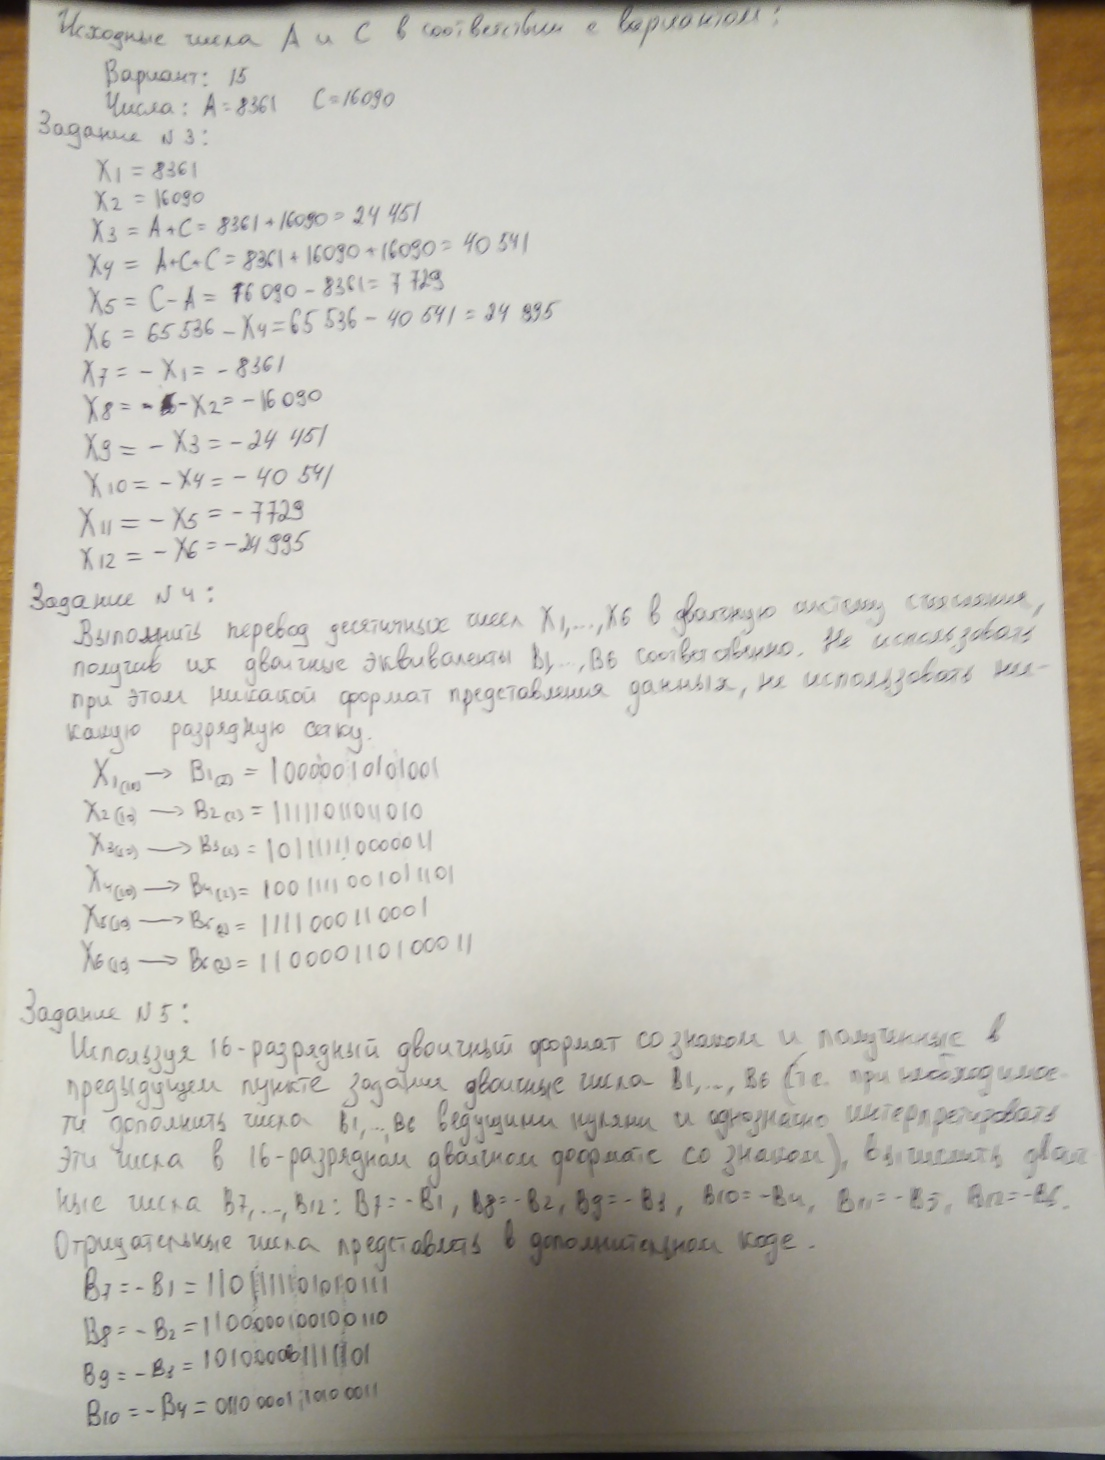
\includegraphics[scale=1,2]{2.jpg}
\end{multicols}
    